\section{Schutzziele}
\label{sec:schutzziele}

Nachdem wir bisher auf die Architektur und die Kommunikation von Microservices eingegangen sind, betrachten wir in diesem Abschnitt die Angriffspunkte einer solchen Infrastruktur. Explizit werden dazu Schutzziele der Informationssicherheit betrachtet. Diese sind ein guter Maßstab dafür, ob bestimmte Angriffe gegen ein Informationssystem möglich sind oder nicht. In dieser Arbeit werden wir für drei Ziele Schutzmechanismen vorschlagen, welche für Microservices in Betracht gezogen werden können. Die ausgewählten Schutzziele spielen dabei eine besondere Relevanz in verteilten Systemen. 

Zunächst werden wir daher in \autoref{subsec:vertraulichkeit} auf das Ziel der Vertraulichkeit eingehen. Weitergehend setzt sich \autoref{subsec:integrität} mit der Integrität und zuletzt \autoref{subsec:verfügbarkeit} mit der Verfügbarkeit von Informationen innerhalb eines Microservice-Netzwerks auseinander.


\subsection{Vertraulichkeit}
\label{subsec:vertraulichkeit}

Zur Einführung der drei Schutzziele ziehen wir die Definitionen von \citeauthor{Bedner+10} zurate, um auf diese näher eingehen zu können. Zunächst widmen wir uns der Vertraulichkeit.

„Informationsvertraulichkeit ist bei einem IT-System gewährleistet, wenn die darin enthaltenen Informationen nur Befugten zugänglich sind. Dies bedeutet, dass die sicherheitsrelevanten Elemente nur einem definierten Personenkreis bekannt werden. Dazu sind Maßnahmen zur Festlegung sowie zur Kontrolle zulässiger Informationsflüsse zwischen den Subjekten des Systems nötig (Zugriffsschutz und Zugriffsrechte), sodass ausgeschlossen werden kann, dass Informationen zu unautorisierten Subjekten ‚durchsickern‘.“ \cite{Bedner+10}

Für eine Microservice-Architektur betrifft dies vor allem die Kommunikation zwischen den einzelnen Microservice-Instanzen. Um diese für beide Gesprächspartner abzusichern werden zwei verschiedene Verfahren vorgestellt, zum einen die Handshake-basierte Authentifikation, bei der sich beide Gesprächspartner einander vorstellen, und die Token-basierte Authentifikation, bei welcher ein Geheimnis, ein sogenanntes „Token“, die Inhalte der Kommunikation quittieren und belegen.


\subsubsection{OAuth-basierte Autorisierung}

Als erstes diskutieren wir ein Handshake-basiertes Autorisierungsverfahren. Im Webumfeld ist das populärste das bereits zuvor angesprochene OAuth-Framework. Es ist aufgenommen worden von der \textit{Internet Engineering Task Force} (IETF). Die Spezifikation für die 2012 veröffentlichte Version 2 des OAuth-Frameworks ist in den \textit{Request for Comments} (RFC) Nummer 6749 der IETF zu finden. Es ist insbesondere für \textit{Single-Sign-On}-Dienste geeignet; also in den Fällen, bei denen man für verschiedene Dienste die gleichen Zugangsdaten verwenden möchte. \cite{RFC6749}

\begin{figure}[h]
	\centering
	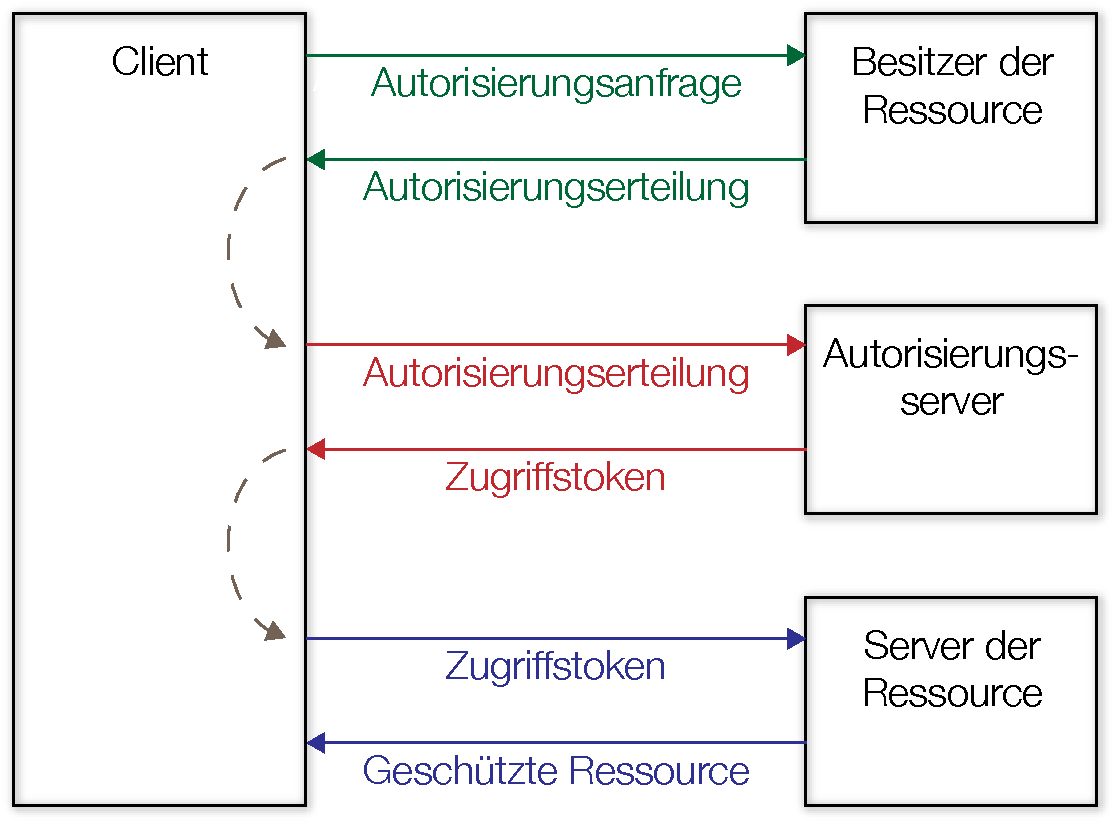
\includegraphics[width=.52\linewidth]{img/OAuth2}
	\caption{Protokollablauf bei OAuth 2 (übersetzt aus RFC 6749).}
	\label{fig:oauth2}
\end{figure}

Zunächst wird aufgezeigt, wie eine Autorisierung mithilfe von OAuth 2 stattfinden kann, um auf Zugriff auf eine externe Ressource zu erhalten. Ein solcher Ablauf ist in \autoref{fig:oauth2} dargestellt. Eine Applikation, die auf die Ressource zugreifen möchte, fungiert dabei als Client. Vorab muss sich dieser beim Besitzer der Ressource eine Autorisierung erteilen lassen. Der Besitzer ist eine Entität, welche über die Informationen der erfragten Ressourcen verfügen kann. Etwa ist dies ein Benutzer oder eine Organisation, deren Details abgefragt werden.

Erteilt der Besitzer die Autorisierung, kann der Client dessen Quittung nutzen um einen Autorisierungsserver zu kontaktieren. Dieser verwaltet die Zugriffe auf die von ihm angebotenen Ressourcen. Sobald der Client die Autorisierungserteilung vorgelegt hat, stellt der Server ein Zugriffstoken aus. Dieser hat dabei die Möglichkeit, die Gültigkeit des Tokens zeitlich zu begrenzen und regelmäßige Aktualisierungen anzufordern. 

Abschließend kann der Client mithilfe eines Zugriffstokens nun auf die Ressourcen zugreifen, welche dem Besitzer gehören und dem Client freigegeben wurden. Dies können verschiedene Orte oder auch schreibende Zugriffe sein. Damit bietet OAuth für Microservices eine gute Möglichkeit, einen Autorisierungsservice anzubieten, über den Tokens für die anderen Microservices angefordert werden können. Im Folgenden stellen wir ein leichtgewichtiges Verfahren vor, welches ähnlich funktioniert.


\subsubsection{JWT-basierte Authentifikation}

Das zuvor gezeigte OAuth-Verfahren offenbart durch seinen Aufbau, dass wir bereits eine recht komplexe Infrastruktur zur Verfügung stellen müssen, um das Framework umzusetzen: drei Applikationen, welche über Formulare mit dem Benutzer interagieren und zusätzlich mit einer Datenbank in welcher die Benutzerdaten abgelegt werden müssen.

Wenn man daher eine Authentifizierung etwas minimaler aufbauen möchte, bieten sich daher \textit{JSON Web Tokens} (JWT) an. Bei diesen können beliebige Informationen encodiert werden, die mithilfe eines Schlüssels zertifiziert werden, um dessen Ursprung zu bestätigen und die Unversehrtheit zu schützen. Diese Technologie hat es im Mai 2015 ebenfalls geschafft, Bestandteil der IETF-Spezifikationen zu werden und ist als RFC mit der Nummer 7519 zu finden. \cite{RFC7519}

Ein JWT besteht aus drei Informationen: Zunächst wird ein Header übertragen, welcher den verwendeten Algorithmus zur Kodierung der Signatur enthält und den Typen des Tokens expliziert; derzeit ist hierfür nur „JWT“ zulässig. Als nächstes folgen die Daten, welche übertragen werden sollen. Diese werden in Form eines JSON benutzt. Die Daten und der Header werden Base64-Kodiert und durch einen Punkt getrennt. Abschließend wird eine Signatur auf Basis dieses Datums berechnet. Dazu wird der im Header deklarierte Algorithmus, entweder \textit{HMAC} oder \textit{RSA}, benutzt. Die Signatur wird nach einem weiteren Punkt an das bisher berechnete Datum gehängt und bildet damit das vollständige Token. Ein Beispiel zeigt \autoref{fig:jwt}.

\begin{figure}[b]
	\centering
	{\tt \textcolor{red}{
			eyJhbGciOiJSUzI1NiIsInR5cCI6IkpXVCJ9}.\textcolor{violet}{eyJ0aG\\
			VtYSI6Ik1pY3Jvc2VydmljZXMgdW5kIFNpY2hlcmhla\\
			XQiLCJzZW1pbmFyIjoiS29tcG9uZW50ZW4sIEFnZW50\\
			ZW4gdW5kIFdvcmtmbG93cyBpbiB2ZXJ0ZWlsdGVuIFN\\
			5c3RlbWVuIn0}.\textcolor{blue}{ASG6OtMb3J30KpwY956UQYAwobI3mm\\
			jH\_7jeUtDEBbTlJmwv632Iw9zIZCfh17h0LZrX3Bny\\
			lJQsaF05bZLejzs-x-wbiTvQxct41Pt0mBlRGKphmK2\\
			hMByfBsrsPbRLpcwpotESsUx6T9FmqsMOXOyBC9RVlL\\
			z9h-6XHFg7hls}}
	\caption{Ein \textit{JSON Web Token}. In Rot ist der Header angegeben, Violett gibt die übertragenen Daten an (Thema und Seminar dieses Aufsatzes) und in Blau ist die in \textit{RSA}-kodierte Signatur enthalten.}
	\label{fig:jwt}
\end{figure}

Verwendet man zur Kodierung den \textit{HMAC}-Algorithmus, so wird ein Geheimnis benutzt, welches nur dem JWT-generierenden Knoten bekannt ist. Bei \textit{RSA} ist es hingegen möglich, ein Schlüsselpaar aus privatem und öffentlichem Schlüssel zu verwenden. Dies ist insbesondere für Microservice-Umgebungen interessant, denn so kann einem Microservice, der lediglich für das Anmelden zuständig ist, der private Schlüssel zum Erstellen des Tokens bekannt sein. Allerdings kann allen Microservices hingegen der öffentliche Schlüssel vorliegen – so kann jeder Microservice beim Eintreffen einer Nachricht die Gültigkeit des Tokens überprüfen und im Falle einer Fälschung die Weiterverarbeitung verweigern.

Das nächste Schutzziel, welchem sich dieser Aufsatz widmen wird, ist die Integrität der zu übertragenen Daten zu schützen. JWT kann, wie wir angegeben haben, auch dazu verwendet werden, würde allerdings so für größere Datenmengen zweckentfremdet werden.


\subsection{Integrität}
\label{subsec:integrität}

Neben der Gewissheit, den Sender einer Nachricht zurückverfolgen zu können, interessiert uns als empfangendes System im Folgenden, auch über deren Inhalt eine Aussage treffen zu können. Diese wird durch das Schutzziel der Integrität abgedeckt und wie folgt definiert.

„Integrität oder Unversehrtheit bedeutet zweierlei, nämlich die Vollständigkeit und Korrektheit der Daten (Datenintegrität) und die korrekte Funktionsweise des Systems (Systemintegrität). Vollständig bedeutet, dass alle Teile der Information verfügbar sind. Korrekt sind Daten, wenn sie den bezeichneten Sachverhalt unverfälscht wiedergeben. Die Integrität bedeutet, dass Daten im Laufe der Verarbeitung oder Übertragung mittels des Systems nicht beschädigt oder durch Nichtberechtigte unbefugt verändert werden können. Beschädigungs- oder Veränderungsmöglichkeiten sind das Ersetzen, Einfügen und Löschen von Daten oder Teilen davon.“ \cite{Bedner+10}

Wir gehen zunächst auf ein Verfahren ein, um die Datenintegrität zu schützen und werden daraufhin Möglichkeiten zum Schutze der Systemintegrität in Microservices aufzeigen.

\subsubsection{Datenintegrität}

Ein besonderes Problem, welches durch die lose Kopplung der Microservice-Instanzen entsteht, ist, dass die Daten zur Weiterverarbeitung abhör- und manipulierbare Wege über standardisierte Protokolle wählen müssen. Wie bereits festgestellt, erfolgt die Kommunikation etwa über REST und damit über HTTP. 

Eine Lösung, die sich hier anbietet, sind Verschlüsselungsverfahren. Das oben angesprochene Framework \textit{Kubernetes} beispielsweise verteilt unter allen Knoten Zertifikate, die ausschließlich im Container-Netzwerk bekannt sind. So können HTTPS-Verbindungen zwischen den Microservice-Instanzen hergestellt werden, die dank AES-Verschlüsselung nicht mehr abgehört oder manipuliert werden können.

Weitere Protokolle, um komplexeren Anforderungen zu genügen, sind das verschlüsselte \textit{WebSocket}-Protokoll WSS oder das sicheres FTP, sprich SFTP. Eine Verbindung via \textit{WebSockets} bietet ohnehin die Möglichkeit an, vor dem Senden der Daten eine Verschlüsselung zu installieren. Allerdings ist hier zu beachten, dass diese im Browser zurückverfolgt werden kann. Eine SFTP-Verbindung funktioniert über das SSH-Protokoll, welches verschiedene Möglichkeiten zur sicheren Kommunikation bietet; etwa auch wie bei JWT mit einem Schlüsselpaar aus öffentlichem und privatem Schlüssel.

\subsubsection{Systemintegrität}

Neben der Integrität der Daten ist es auch wichtig, die Integrität eines Microservice-Systems zu wahren. Ein Ansatz dafür ist zum Beispiel das automatisierte Testen. Wie dieses auf die lose Kopplung einer Microservice-Architektur angewendet werden kann, um die korrekte Arbeitsweise jener zu validieren, wird in dem Vortrag \cite{Clemson14} geschildert. In diesem wird gezeigt, wie Integrationstests genutzt werden können, um das Zusammenspiel mehrerer Microservices zu testen.

\begin{figure}[h]
	\centering
	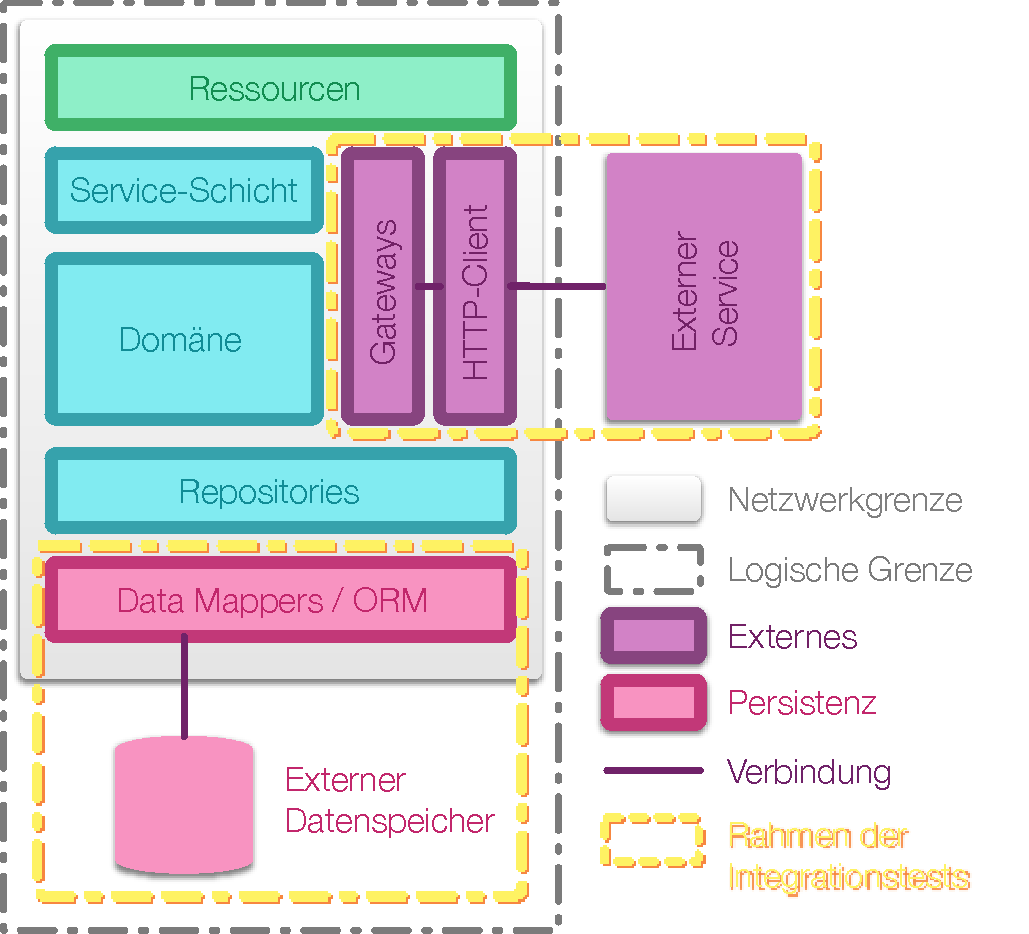
\includegraphics[width=.6\linewidth]{img/inte}
	\caption{Rahmen der Integrationstests in einer Microservice-Architektur (übersetzt aus Clemson, 2014).}
	\label{fig:integrationstests}
\end{figure}

Bei einem Integrationstest werden bestimmte Teile eines gesamten Informationssystems als abgeschlossenes Subsystem getestet. So können Fehler oder Schwächen einer Schnittstelle entdeckt werden und es wird verhindert, dass bei zunehmender Änderung der einzelnen Komponenten bestimmte Abkommen nicht mehr eingehalten sind, was zu Laufzeitfehlern führen könnte.

\autoref{fig:integrationstests} zeigt eine exemplarische Microservice-Architektur auf. Hierbei sind die Bereiche hervorgehoben, bei denen die Integrationstests unseres Dienstes ansetzen sollen. Der untere Abschnitt zeigt \textbf{Persistent-Integrationstests}. Dabei wird getestet, ob ein Microservice korrekt mit einer Datenbank, einem Cache oder der Abstraktion einer solchen arbeitet. Weitergehend bildet der rechte Bereich \textbf{Gateway-Integrationstests} ab. Hier können Fehler bei der Umsetzung der verwendeten Protokolle, \textit{Message Queues} oder auch in der JWT-Implementierung aufgedeckt werden. Außerdem wird festgestellt, ob ein Microservice die essentiellen Daten überträgt, die er vorgibt zu senden.

Mit der Integration verlassen wir den Bereich der softwaretechnisch lösbaren Sicherheitsprobleme und widmen uns im Folgendem dem letzten Schutzziel, welches wir betrachten werden, nämlich das der Verfügbarkeit eines Microservice-Systems.


\subsection{Verfügbarkeit}
\label{subsec:verfügbarkeit}

Zuletzt widmen wir uns in dieser Arbeit der Verfügbarkeit als Schutzziel eines Microservice-Systems. Dabei ist die Maxime unseres Systems, nach Möglichkeit permanent erreichbar zu sein. Die folgende Definition erläutert den Verfügbarkeitsbegriff ausführlicher.

„Die Verfügbarkeit betrifft sowohl informationstechnische Systeme als auch die darin verarbeiteten Daten und bedeutet, dass die Systeme jederzeit betriebsbereit sind und auf die Daten wie vorgesehen zugegriffen werden kann. Zum einen muss die Datenverarbeitung inhaltlich korrekt sein und zum anderen müssen alle Informationen und Daten zeitgerecht zur Verfügung stehen und ordnungsgemäß verarbeitet werden.“ \cite{Bedner+10}

Microservices sind, wie bereits einleitend erwähnt, sehr einfach horizontal zu skalieren. Dadurch haben wir die Möglichkeit, viele parallele Instanzen zu benutzen welche die gleiche Aufgabe erfüllen. Dies machen wir uns im zunächst genannten Lösungsansatz zunutze. Daraufhin erläutern wir einen neuartigen Ansatz, wodurch dieses Prinzip sogar noch weiter verbessert werden kann, um eine noch bessere Verfügbarkeit zu erzielen.

\subsubsection{Redundanz und Lastverteilung}

Durch die lose Kopplung und die harten Grenzen können Microservice-Instanzen ohne weitere Mühen vervielfältigt werden. Da die Kommunikation über Webtechnologie erfolgt, können Microservices auch über Systemgrenzen hinweg auf mehrere Rechnerknoten verteilt werden. Das heißt wir haben zunächst die Möglichkeit, einen Datenknoten mit allen Microservices durch Aufrüsten der Hardware zu skalieren und können anschließend unter vertretbarem Aufwand einen zweiten Knoten mit dem ersteren verbinden, um auf diesem weitere Instanzen auszuführen.

Haben wir mehrere Instanzen eines Microservices, benötigen wir einen Entscheider, welcher einen ankommenden Zugriff einer Instanz zuordnet. Einen solchen Entscheidungsvorgang nennen wir \textbf{Lastverteilung} (vom Englischen \textit{Load Balancing}). Zuvor bereits wurde eine der populärsten Implementierungen dieser angesprochen, nämlich die Software \textit{HAProxy}. Es gibt diverse Strategien, nach denen Lastverteilung ablaufen kann, und welche auch durch \textit{HAProxy} unterstützt werden.

\begin{itemize}
	\item Die einfachste Strategie ist eine, welche auf Basis des \textbf{Zufalls} entscheidet, welcher Instanz ein Auftrag zugeordnet wird. Allerdings wird dabei nicht berücksichtigt, wie groß die Aufträge sind, sodass in ungünstigen Fällen eine Instanz häufiger arbeitsintensive Aufträge erhält als andere.
	
	\item Als zweites kann auch \textbf{Sharding} in Betracht gezogen werden. Dafür teilen wir den ankommenden Datenbestand nach bestimmten Prinzipien auf möglichst gleichgroße Teilmengen auf. Etwa kann auf Basis des Alphabets (A-K, L-R, S-Z) oder eines Zahlenbereichs ein \textit{Shard} bestimmt werden. Eine Microservice-Instanz ist dann für einen solchen \textit{Shard} verantwortlich.
	
	\item Wir können die Last auch abhängig von der \textbf{Auslastung} eines jeweiligen Knoten verteilen. Dazu fragt die Lastverteilung die in Betracht gezogenen Knoten regelmäßig, wie viele Aufträge diese zur Zeit bearbeiten und weist ihnen dementsprechend weitere zu. Problematisch bei diesem Verfahren ist, dass es zusätzliche last erzeugt und technisch anspruchsvoller als die beiden zuvor erklärten Strategien ist.
\end{itemize}

Lastverteilung ermöglicht es der Architektur, mehrere Instanzen eines Microservices zu verwenden. Wie auch immer ist dabei zu erwähnen, dass wir einen neuen Flaschenhals erzeugen, da jegliche Microservice-Zugriffe zunächst der Lastverteilung anvertraut werden. Dies stellt einen sogenannten \textit{„Single Point of Failure“} dar. Im Folgenden zeigen wir daher eine Verbesserung des oben genannten Prinzips auf.

\subsubsection{Clientseitige Lastverteilung}

In dem Blog-Beitrag \cite{Li15} wird ein neuartiger Ansatz motiviert, welcher die Verfügbarkeit von Lastverteilung verbessert. Dies ist notwendig, da, wie eben festgestellt, der Last-verteilende \textit{Load Balancer} einen Flaschenhals darstellt. Sollte dieser ausfallen, ist das System nicht mehr erreichbar.

\begin{figure}[h]
	\centering
	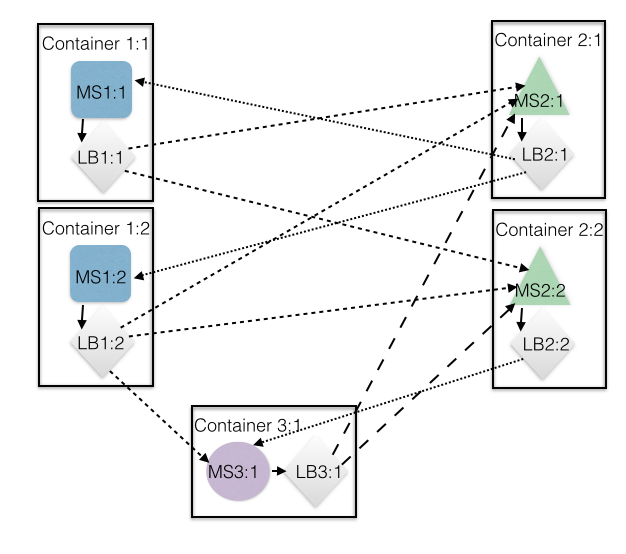
\includegraphics[width=.55\linewidth]{img/clientloadbal}
	\caption{Schematische Darstellung von clientseitiger Lastverteilung (aus Li, 2015). Drei heterogene Microservices (MS) verfügen jeweils über eine Lastverteilung (LB), welche alle Instanzen anderer Microservices kennt.}
	\label{fig:clientseitige_lastverteilung}
\end{figure}

Abhilfe für dieses Problem stellt der folgende clientseitige Lastverteilungsdienst dar. Diese funktioniert so, dass jeder Microservice, welcher auf die Dienste anderer angewiesen ist, über seine eigene Lastverteilung verfügt. Ein solcher Aufbau ist in \autoref{fig:clientseitige_lastverteilung} schematisiert: Ein Microservice verfügt über seinen eigenen \textit{Load Balancer}, an welchen er seine ausgehende Kommunikation exklusiv leitet. Dieser kennt alle anderen Microservice-Instanzen und kann daher Nachrichten an diese weiterleiten.

Die von \citeauthor{Li15} entwickelte Grundstruktur \textit{„Baker Street“}\footnote{\textit{Baker Street} ist unter Apache-Lizenz 2 veröffentlichte freie Software, siehe \url{http://bakerstreet.io/}.} ist eine Umsetzung dieser Architektur. Kern dieser sind drei folgenden Komponenten.

\begin{itemize}
	\item Der \textit{HAProxy}-basierte \textit{Load Balancer} \textbf{Sherlock} welcher lokal jeder Microservice-Instanz beiwohnt. Er findet heraus, wohin Verbindungen von dieser Instanz wandern sollen.
	
	\item Der \textit{Health Checker} \textbf{Watson} über den ebenfalls jede lokale Instanz verfügt. Er übermittelt den Zustand des Microservices und meldet diesen ebenfalls initial an.
	
	\item Zuletzt gibt es das \textbf{Datawire-Verzeichnis}, ein leichtgewichtiger globaler Diensterkundungs"=Mechanismus, welcher Informationen von jeder Watson-Instanz erhält und Verfügbarkeitsänderungen zu jeder lokalen Sherlock-Instanz weiterleitet.
\end{itemize}

Mit diesen drei Komponenten haben wir eine hohe Verfügbarkeit für die Grundstruktur unserer Microservice-Systems erzielt: Fällt ein Knoten mitsamt seines \textit{Load Balancers} aus, weiß das \textit{Datawire}-Verzeichnis Bescheid und die Anwendung bleibt verfügbar, da es keinen zentralen Knoten mehr gibt, der nicht antworten könnte.

Damit haben wir für alle drei Schutzziele der Vertraulichkeit, der Integrität und der Verfügbarkeit ausreichende Lösungsmöglichkeiten aufgezählt und schließen im folgenden Abschnitt die Ausarbeitung mit einer Zusammenfassung der Ergebnisse.